\chapter{Einleitung}
Viele Menschen nutzen das Internet, um sich über Restaurants, deren Speisekarten und Mittagsmenüs zu informieren.
Häufig werden dabei von einer Person die Websites der Restaurants ihres Vertrauens aufgerufen und geprüft, was heute auf dem Menüplan steht.
Diese Tätigkeit nimmt einige Zeit in Anspruch.
Es ist mühsam, mehrere Websites aufzurufen, deren Menüseiten zu suchen und zu prüfen.\\
Die Idee dieser Arbeit ist das Erstellen einer Suchmaschine, über welche sich Restaurant-übergreifend Menüs und Speisen suchen lassen.
Die Grundlage einer solchen Suchmaschine sind die Websites von Restaurants in Kombination mit Informationen wie z.B. dem Standort.
Um diese Websites automatisiert abzufragen und zu speichern, ist ein sogenannter Webcrawler nötig.
\begin{figure}[H]
	\centering	
	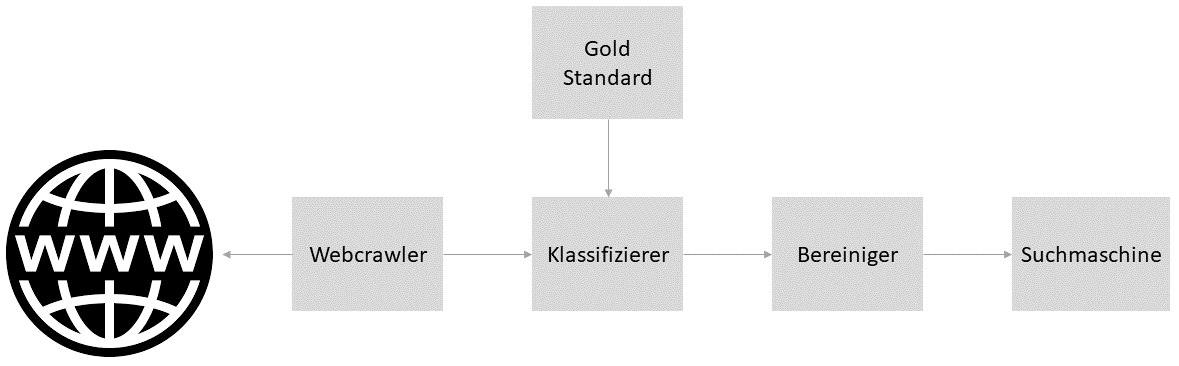
\includegraphics[width=1\columnwidth,keepaspectratio]{img/Ablauf_Einleitung.png}
	\caption{Pipeline}
	\source{Eigene Darstellung}
	\label{fig:ablauf_einleitung}
\end{figure}
Dieser bildet die erste Komponente einer Pipeline zur Verrichtung dieser Aufgabe, welche in \cref{fig:ablauf_einleitung} dargestellt ist.
Da der Webcrawler jedoch alle möglichen Seiten speichert, also z.B. auch die Datenschutzerklärung eines Restaurants, müssen diese klassifiziert werden, denn nur Webseiten mit Informationen über Menüs und Speisen sollen in der Suchmaschine gezeigt werden.
Dazu wird eine weitere Komponente, der Klassifizierer, benötigt.
Dieser entscheidet mittels Algorithmen, ob die Seite Menüinformationen beinhaltet oder nicht.
Um eine Aussage machen zu können, wie gut dieser Klassifizierer ist, braucht es zudem einen Testdatensatz, der sogenannte Gold Standard.
Dieser enthält sowohl positive als auch negative von Hand klassifizierte Beispiele von Restaurant-Webseiten.
Als Menüseiten klassifizierte Webseiten müssen in eine einheitliche Form gebracht werden und mit Informationen über das Restaurant, wie z.B. dem Standort, versehen werden.
Dazu wird eine dritte Komponente, der Bereiniger benötigt.
Zum Schluss werden diese Daten in der für den Benutzer zugänglichen Suchmaschine verwaltet.  
